\chapter{Grundlagen und Methoden}
Im \textbf{Kapitel 2} werden die \textbf{Grundlagen und Methoden} geklärt.


\section{Analyse des vorhandenen Systems}
Text

\subsection{Begriffe}
Text

\subsubsection{Echtzeitdaten}
Text

\subsubsection{Energietechnologie}
Text

\subsubsection{Energiesystem}
Text

\subsubsection{Front-End}
Text

\subsubsection{Back-End}
Text








\section{Anforderungen an das Produkt}
Text

\subsection{Schutz von vertraulichen Informationen}
Text

\subsection{Statistische Auswertung}
Text



\section{Architektur des Zielsystems}
Text

\subsection{Endgeräte}
Text

\subsection{Serverseitig}
Text

\subsection{Clientseitige Interaktion des Benutzers}
Text

\subsection{Framework}
Die Wahl des Frameworks ist für die Umsetzung des Projekts entscheidend. Unter dem Begriff Framework versteht man eine Art Programmiergerüst, die es dem Programmierer deutlich erleichtert, ein Produkt zu erstellen. Jedes Framework bietet spezielle Lösungen und Lösungsansätze an und damit hat jedes einzelne sein eigenes Einsatzgebiet. In den nachfolgenden Unterkapiteln werden mögliche Frameworks für die Umsetzung des Projekts kurz erklärt. In \ref{sec:Entscheidung des Frameworks} wird genauer darauf eingegangen, welches Framework gewählt wurde und aus welchem Grund.

\subsubsection{Laravel}
Das PHP-Framework Laravel, welches 2011 entwickelt wurde, basiert auf dem MVC Muster\footnote{wird in  \autoref{sec:MVC} genauer erläutert} und bietet damit eine sehr gute Strukturierung und Übersicht beim Arbeiten. Laravel wird in den meisten Fällen als Back-End Framework verwendet. Die meisten Projekte werden mit Laravel im Back-End in Kombination mit Vue.js im Front-End umgesetzt. Genauere Informationen  zu Vue.js sind im Kapitel 2.6.3 nachzulesen. Laravel bietet jedoch die Möglichkeit, im Back- als auch im Front-End verwendet zu werden. Es lässt sich in folgende Einzelteile strukturieren:

\begin{itemize}
	\item Migrations 
	\item Views
	\item Controller 
	\item Models
	\item Routen 
\end{itemize}

Migrations sind die Abbildung der Tabellenstruktur und ermöglichen es, bei richtiger .env Datei Konfiguration, mit artisan Befehlen, ganz einfach eine Datenbank und die dazugehörigen Tabellen zu erstellen und diese auch genauso einfach wieder zu löschen oder zu leeren. Views fungieren als visueller Gliederungspart zwischen den Controllern und den Benutzern. In ihnen wird alles, was auf der Oberfläche ersichtlich ist, ausprogrammiert und gestaltet. Controller bilden die Verbindung zwischen den Views und den Models und ermöglichen es dem Benutzer, Daten mithilfe eines Zugriffs auf das Models zu verändern. Models bilden die Datenstruktur ab und ermöglichen den Zugriff auf die Daten und die Änderung dieser. Routen vermitteln die Benutzerabfrage von der View mit dem dazugehörigen Controller und werden in der Datei “web.php” definiert. Der ganze Prozess ist in \autoref{fig:Laravel MVC} visuell dargestellt. 
\begin{figure}[h]
	\centering
	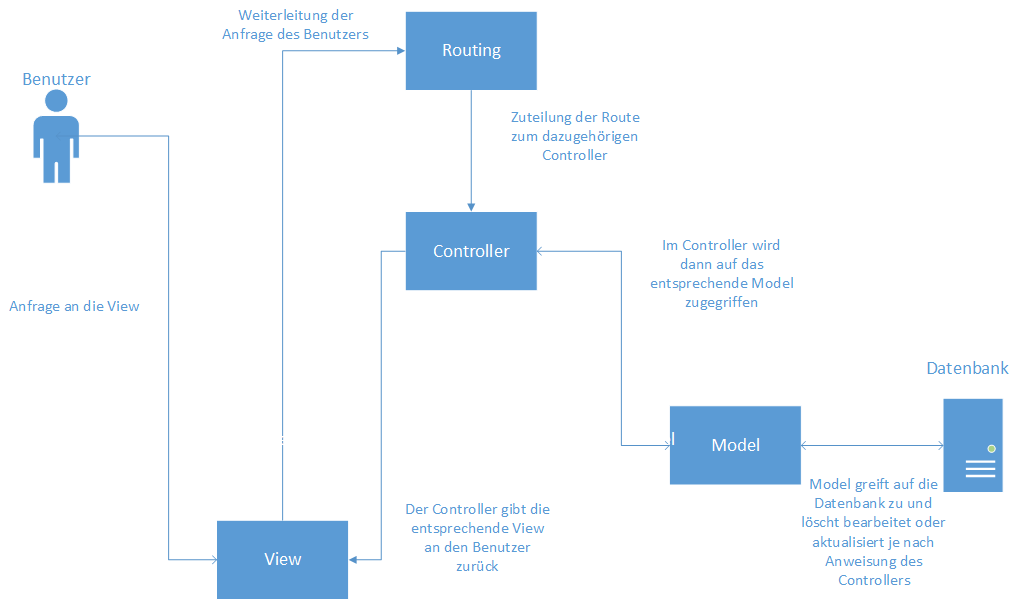
\includegraphics[height=8cm,width=15cm]{images/LaravelMVC}
	\caption{Laravel MVC}
	\label{fig:Laravel MVC}
\end{figure}
\subsubsection{Angular}
\subsubsection{ASP.NET}
\subsubsection{React}
\subsubsection{Entscheidung des Frameworks}\label{sec:Entscheidung des Frameworks}


\subsection{Front-End Templates}
\subsubsection{Bootstrap}
\subsubsection{Tailwind.css}
\subsubsection{Vue.js}
\subsubsection{Entscheidung des Front-End Templates}


\subsection{Verbindung der Datenbank mit Laravel}
\subsubsection{Laravel .env Datei }
\subsubsection{Migrations}
\subsubsection{Seeder / Factories}
\subsubsection{Datenübergabe in Laravel}


\section {Visuelle Darstellung der Energiesysteme und Energietechnologien }

\subsection{Kartendienste}

\subsubsection{Google Maps}
\subsubsection{OpenStreetMap}

\subsection{Geoinformationssystem }

\subsection{CSS-System}

\subsection{Auswahl des Anbieters}


\section{Berechtigungssystem Benutzer}

\subsection{Benutzerrollen}

\subsubsection{Administrator}
\subsubsection{Mitarbeiter}
\subsubsection{öffentlicher Benutzer}

\subsection{Berechtigungen in Laravel}


\section{Ui/Ux Design}

\subsection{Wireframe}

\subsection{Persona}


\section{Template Layout}

\subsection{Platzhalter Yield}

\subsection{Sections}
\subsection{Einbindung der definierten Sections}


\section{Laravel Befehle}

\subsection{Migration Befehle}
\subsection{Seeder und Factory Befehle}
\subsection{Model und Controller Befehle}
\subsection{Starten des Laravel Develop Servers}
\subsection{Befehle nach dem Git Pull} 



\chapter{Ergebnisdokumentation }
Im \textbf{Kapitel 3} wird die \textbf{Ergebnisdokumentation} geklärt.

\section{Laravel }
Text

\subsection{Installation}
Text

\subsection{Bootstrap Einbindung}
Text
\subsection{Grafana Einbindung}
Text

\subsection{MVC}\label{sec:MVC}
Text
\subsubsection{Model}
Text
\subsubsection{View}
Text
\subsubsection{Controller}
Text


\section{Datenbankanbindung in Laravel}
Text

\subsection{Datenbank Anmeldeinformationen}
Text

\subsection{Mail Server Konfigurationen}
Text

\subsection{Migrations}
Text


\section{Routen in Laravel}
Text

\subsection{Resource Routen}
Text

\subsection{GET Routen}
Text

\subsection{Auth Routen}
Text


\section{Datenbankdesign}
Text

\subsection{Erstellen eines neuen Schemas}
Text

\subsubsection{ER-Model}
Text

\subsubsection{Fremdschlüssel}
Text


\section{Corporate Design}
Text

\subsection{Vorschläge}
Text

\subsection{Änderungsvorschläge}
Text

\subsection{Finales Design}
Text

\subsection{Definierte Farben}
Text

\subsection{Überschriften}
Text

\subsection{Interaktionsfarben}
Text

\subsection{Schriftarten}
Text

\subsection{Schriftgrade}
Text

\subsection{Logo}
Text

\subsection{Verwendete Icons und deren Bedeutungen}
Text

\subsection{Map Icons}
Text

\subsection{Icons in Formularen}
Text

\subsection{Icons im DataTable}
Text

\subsection{Buttons}
Text

\subsection{Tabelle mit generellen Informationen über einzelne HTML Elemente}
Text

\subsection{Datenformate}
Text



\section{Weboberfläche}
Text

\subsection{Backend}
Text
\subsubsection{Energiesystem Erstellen}
Text

\subsubsection{Energiesystem Bearbeiten}
Text

\subsubsection{Energiesystem Löschen}
Text

\subsubsection{Energietechnologie Erstellen}
Text

\subsubsection{Energietechnologie Bearbeiten}
Text

\subsubsection{Energietechnologie Löschen}
Text

\subsubsection{Benutzerverwaltung}
Text

\subsubsection{Adresssuche}
Text


\subsection{Front-End}
Text

\subsubsection{Home}
Text

\subsubsection{Energiesysteme}
Text

\subsubsection{Galerie}
Text

\subsubsection{Impressum}
Text

\subsubsection{Datenschutz}
Text

\subsubsection{Registrierungsseite}
Text

\subsection{Login}
Text

\subsection{Registrierung}
Text

\subsection{Kartendienst Funktionalitäten}
Text

\subsubsection{Auswählen eines Energiesystems}
Text
\subsubsection{Abwählen eines Energiesystems}
Text

\subsection{Anzeige von Energiesystemen und Energietechnologien auf der Karte}
Text
\subsubsection{Energiesysteme Marker auf der Karte platzieren}
Text
\subsubsection{Energietechnologien Marker auf der Karte platzieren}
Text

\subsection{Layoutvorlage der Website}
Text



\section{DataTable}
\definecolor{mygray}{RGB}{252,251,244}
\renewcommand{\lstlistingname}{Quellcode}

\begin{lstlisting}[
	caption={Funktion Blade.php Zeile 1-2},
	label=Code,
	language=octave,
	numbers=left,
	firstnumber=100,
	numberfirstline=false,
	backgroundcolor=\color{mygray},
	basicstyle=\footnotesize=15,
	keywordstyle=\color{blue}
	]
	
	$EnSys = EnSys::find($id);
	$data = DB::table('EnSys')->get();
	//Kommentar
	$EnTech = EnTech::where('enSys_idEnSys', $id)->get();
\end{lstlisting}
\subsection{Individueller DataTable}
Text
\subsection{Sortierfunktion}
Text
\subsection{Suchfunktion}
Text
\subsection{Seitenanzahl}
Text
\subsection{Icons}
Text
\subsection{MoveToMarker}
Text


\section{Galerie Funktionen}
Text
\subsection{Auswahl eines Energiesystems}
Text
\subsection{Energietechnologien des Energiesystems anzeigen}
Text



\section{Grafana}
Text

\subsection{Automatisches Erstellen der Dashboards}
Text

\subsection{Automatisches Erstellen der Panels}
Text

\subsection{Energietechnologien Statistiken anzeigen}
Text



\section{Einbindung von Google Maps}
Text

\subsection{Google Cloud}
Text

\subsection{Google Cloud Platform Account erstellen}
Text

\subsection{Apis aktivieren und einbinden}
Text

\subsection{Individuelle Map erstellen und einbinden}
Text



\chapter{Resümee und Ausblick}
Text


\chapter{Quellen und Literatur}
Text

\chapter{Abbildungsverzeichnis}
Text
\chapter{Tabellenverzeichnis}
Text
\chapter{Codeverzeichnis}
Text


\chapter{Begleitprotokoll gem. § 9 Abs. 2 PrO-BHS}
Text
\section{Begleitprotokoll David Pöchacker}
Text
\section{Begleitprotokoll Marcel Entner}
Text
\section{Begleitprotokoll Tobias Kronsteiner}
Text



\chapter{Anhang}
Text

\section{Verfasser der Kapitel}
Text
\subsection{David Pöchacker}
Text
\subsection{Marcel Entner}
Text
\subsection{Tobias Kronsteiner}
Text


\section{Verwendete Software}
Text
\subsection{Visual Studio Code}
Text
\subsection{Apache WebServer}
Text
\subsection{Composer}
Text
\subsection{Windows Eingabeaufforderung (CMD)}
Text
\subsection{Github VCS und Github Desktop GUI}
Text
\subsection{ phpMyAdmin}
Text
\subsection{Adobe XD}
Text
\subsection{Adobe Photoshop}
Text



\section{Projektplanung}
Text
\subsection{Projektkommunikation}
Text
\subsection{Projektstrukturplan}
Text
\subsection{Verantwortungsmatrix und Aufwandsschätzung}
Text
\subsection{Meilensteinplan}
Text
\subsection{Terminplan}
Text


\section{Inhalt von GitHub}
Text






